\documentclass[border=2pt]{standalone}
\usepackage{garamondx}
\usepackage{pgfplots}
\usepackage{tikz}
\usepgfplotslibrary{units}
\usepackage{filecontents}
\begin{filecontents*}{data}
y,x
0.89567,0.00005
0.73319,0.00004
0.5592,0.00003
0.38137,0.00002
0.1842,0.00001
\end{filecontents*}

\usepackage{xcolor}
\definecolor{redtea}{rgb}{0.6823529412,0.2792156863,0.2666666667}
\definecolor{darkolivegreen}{rgb}{0.33, 0.42, 0.18}
\definecolor{darkbyzantium}{rgb}{0.36, 0.4, 0.33}
\definecolor{darkelectricblue}{rgb}{0.33, 0.41, 0.47}
\definecolor{deepchestnut}{rgb}{0.73, 0.31, 0.6}
\definecolor{azuremist}{rgb}{0.94, 1.0, 1.0}
\usepackage{siunitx}
\usepackage{changepage}


\begin{document}
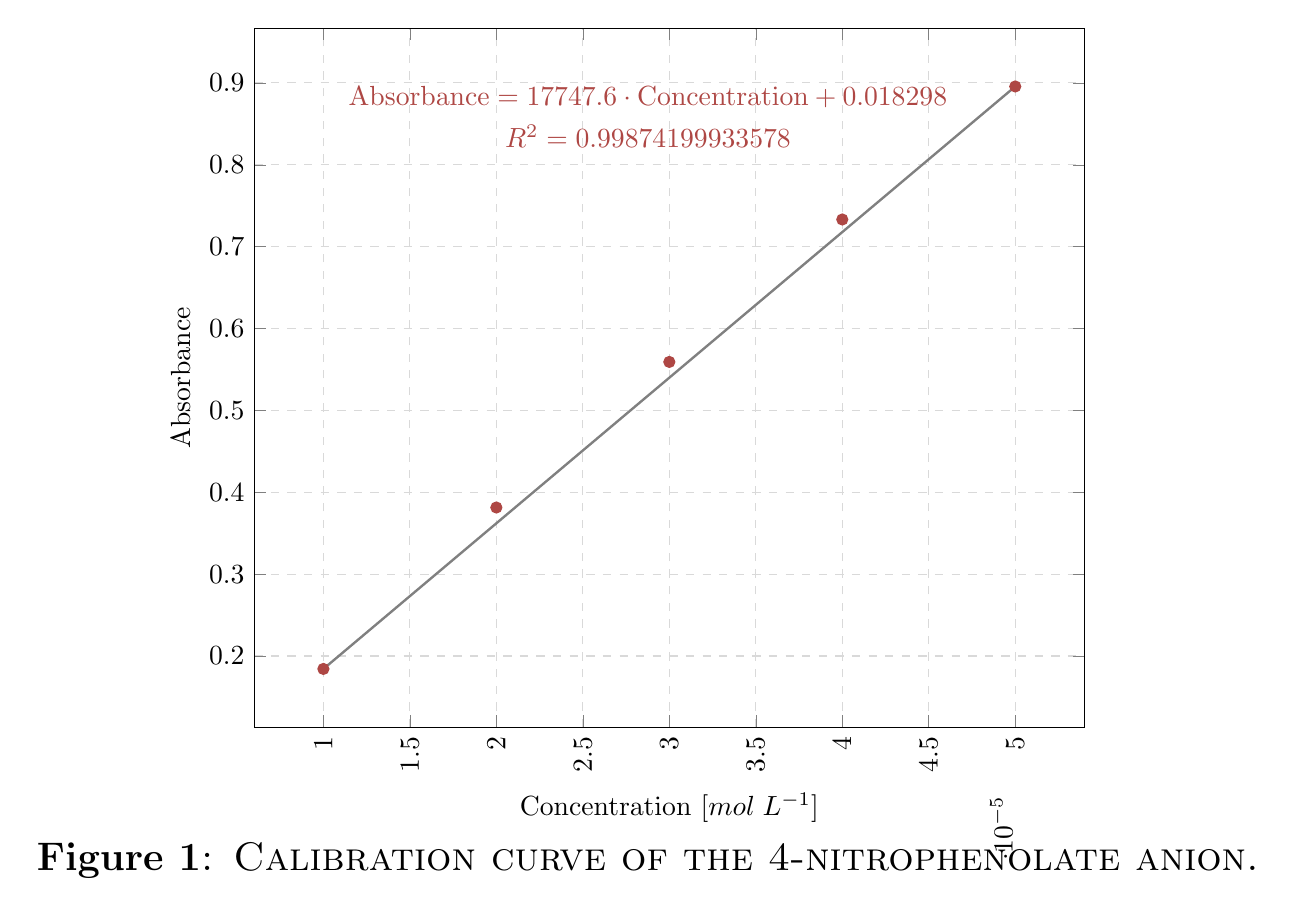
\begin{tikzpicture}
\begin{axis}[
width=\linewidth,
grid=major,
grid style={dashed,gray!30},
xlabel=\raisebox{-2ex}{Concentration $\lbrack mol\;L^{-1}\rbrack$},
ylabel=Absorbance,
x unit=,
y unit=,
legend style={at={(0.5,-0.2)},anchor=north},
x tick label style={rotate=90,anchor=east},
]
%\addplot[redtea] table [col sep=comma,x=x, y=y,mark=*] {data};
\addplot[
color = redtea,
fill = redtea,
mark = *,
only marks
] coordinates {
(0.00005,0.89567)
(0.00004,0.73319)
(0.00003,0.5592)
(0.00002,0.38137)
(0.00001,0.1842)
};
\addplot[
color = gray,
mark = none,
line width=0.2ex
] coordinates {
	(0.00005,0.89567)
(0.00001,0.1842)
};
\end{axis}

\node[redtea] at (5,8) {$\text{Absorbance}=17747.6\cdot \text{Concentration}+0.018298$};
\node[redtea] at (5,7.5) {$R^2=0.99874199933578$};
\node at (5,-1.7) {\Large\scshape\textbf{Figure 1}: Calibration curve of the 4-nitrophenolate anion.};

\end{tikzpicture}
\end{document}


